\documentclass[11pt, a4paper]{report}

\usepackage{geometry}
\usepackage[utf8]{inputenc}
\usepackage[english]{babel}
\usepackage[T1]{fontenc}

\usepackage{graphicx} % Required for including pictures
\usepackage{float} % Allows putting an [H] in \begin{figure} to specify the exact location of the figure
\usepackage{pdfpages}
\usepackage{booktabs}
\usepackage{tabularx}
\restylefloat{table}

\usepackage{tikz}
\usepackage{forest}
\usepackage{caption}
\usepackage{subcaption}
\usepackage{wrapfig} % Allows in-line images such as the example fish picture

\usepackage{lmodern} % load a font with all the characters

\linespread{1.2} % Line spacing

%\setlength\parindent{0pt} % Uncomment to remove all indentation from paragraphs

\graphicspath{{Pictures/}} % Specifies the directory where pictures are stored

\renewcommand{\baselinestretch}{1.3}
\headsep = 10.mm
%%%% CHOOSE MARGINS %%%%

\geometry{hmargin=2.5cm,top=3cm,bottom=2.3cm}
%%%% COMMANDS %%%%
%%%%%%%%%%%%%%%%%%%%%%%%%%%%%%%%%%%%% CHANGE HERE %%%%
\renewcommand\title{UCLCampus: a moblie application for UCL students}
\newcommand\nameone{Arnold \textsc{Moyaux}}
\newcommand\nametwo{Baptiste \textsc{Lacasse}}
\newcommand\options{}
\newcommand\supervisor{Yves \textsc{Deville}}
\newcommand\readerone{Kim \textsc{Mens}}
\newcommand\readertwo{hildeberto \textsc{Mendonça}}
\newcommand\readerthree{Mathieu \textsc{Zen}}
\newcommand\readerfour{Jorge \textsc{Perez Medina}}
\newcommand\years{2015-2016}
%%%% BEGIN %%%%
\begin{document}

%%%% COVER %%%%
\thispagestyle{empty}
\noindent\begin{minipage}{.25\textwidth}
\noindent
\includegraphics[width=3.6cm]{Images/ucl.jpg}
\end{minipage}
\begin{minipage}{.5\textwidth}
\begin{center}
UNIVERSITE CATHOLIQUE DE LOUVAIN
\\~\\~
ECOLE POLYTECHNIQUE DE LOUVAIN
\\~\\~\\~\\~\\~
\end{center}
\end{minipage}
\begin{minipage}{.25\textwidth}
\hfill
\includegraphics[width=3.6cm]{Images/epl.jpg}
\\~\\~\\~\\~
\end{minipage}
\vspace{4.5cm}
\begin{center}
\bfseries{\scshape{\Huge{\title}}}
\end{center}
\vspace{4.5cm}
\begin{minipage}{.5\textwidth}
\begin{tabular}{ll}
Supervisor: & \supervisor
\\ Readers: & \readerone 
\\          & \readertwo 
\\          & \readerthree
\\          & \readerfour
\end{tabular} 
\\~\\~
\end{minipage}
\begin{minipage}{.5\textwidth}
\begin{tabular}{l}
Thesis submitted for the Master's degree
\\ in computer science and engineering
\\ options: \
\\ by : \nameone
\\ 	   \nametwo
\end{tabular}
\end{minipage}
\vfill
\begin{center}
Louvain-la-Neuve
\\ Academic year \years
\end{center}
%%%% END COVER %%%%
%----------------------------------------------------------------------------------------
%	TABLE OF CONTENTS
%----------------------------------------------------------------------------------------

\tableofcontents % Include a table of contents

\newpage % Begins the essay on a new page instead of on the same page as the table of contents 


\chapter{Introduction} % Major section

Brief introduction of the project, the goals and the contents of the rest of the thesis.


\chapter{Background}

In this section, we will look at the different existing technologies relating to the different aspects of our project and will explain the choices we made. // TODO

\section{Cross-platform mobile development tools}

In each of these sections, we will detail the different approaches one could choose to develop a cross-platform moblie applications. We will also present several frameworks using these approaches. We will then compare them and choose one of those approaches for the rest of the project. //TODO
\subsection{The native approach}

The first approach we considered for our project was what we call a native approach. The native approach consists in using the native technology and language for each platform, for instance Java for Android and Objective-C for iOS.  

\begin{table}[H]
\begin{tabularx}{\linewidth}{>{\parskip1ex}X@{\kern4\tabcolsep}>{\parskip1ex}X}
\toprule
\hfil\bfseries Pros
&
\hfil\bfseries Cons
\\\cmidrule(r{3\tabcolsep}){1-1}\cmidrule(l{-\tabcolsep}){2-2}

Best achievable performance\par
Always up-to-date with the latest API\par
Can use any platform\par

&

Low maintainability\par
Harder to find contributors fluent in all technologies\par
Can lead to different versions of the application\par


\\\bottomrule
\end{tabularx}
\caption{Pros and cons of the native approach}
\end{table}

\subsection{The web approach}
A second approach we considered was the web approach. This approach consists in using HTML5 to develop an application that will be usable on any platform.


\begin{table}[H]
\begin{tabularx}{\linewidth}{>{\parskip1ex}X@{\kern4\tabcolsep}>{\parskip1ex}X}
\toprule
\hfil\bfseries Pros
&
\hfil\bfseries Cons
\\\cmidrule(r{3\tabcolsep}){1-1}\cmidrule(l{-\tabcolsep}){2-2}

Can be used on any mobile platform\par
Easy to find contributors fluent in HTML5\par
Easy to maintain\par

&

Doesn't have access to native platform features\par
Harder to implement local storage/security (//TODO NEED BETTER SOURCE)\par
Not as performant as native\par



\\\bottomrule
\end{tabularx}
\caption{Pros and cons of the web approach}
\end{table}
\subsection{The hybrid approach}

The last approach to develop a mobile application is called the hybrid approach. An hybrid app is mostly built using HTML5 and JavaScript and is then wrapped inside a thin native container, giving it access to native features.

\begin{table}[H]
\begin{tabularx}{\linewidth}{>{\parskip1ex}X@{\kern4\tabcolsep}>{\parskip1ex}X}
\toprule
\hfil\bfseries Pros
&
\hfil\bfseries Cons
\\\cmidrule(r{3\tabcolsep}){1-1}\cmidrule(l{-\tabcolsep}){2-2}

Can be used on any mobile platform\par
Easy to find contributors fluent in HTML5 and JavaScript\par
Easy to maintain\par

&

Not as performant as native\par



\\\bottomrule
\end{tabularx}
\caption{Pros and cons of the hybrid approach}
\end{table}

\subsection{Our choice}

\section{Open-source project and code sharing}

In this section, we will explain the choices we made concerning the code sharing platforms we used as well as the licenses we used to protect our work.

\section{Project Management Methodologies}

Here we detail the choices we made as to how we were going to manage de different parts of the project.

\chapter{Functionalities of UCLCampus}

In this part, we will show how we defined the relevant functionalities of our application as well as the user interface.

\section{Choice of functionalities and sections}

\section{User interface}

\chapter{Implementation}

Here we will explain the overall architecture of the application. We will also explain some aspects we considered when implementing the application.

\section{Architecture}

The purpose of the application is to be extensible and easily maintainable. We wanted a programmer can add its functionalities at each level to the application.
For this we thought our implementation as a tree. At the top level we have the application with the settings menu and base configuration after it we have four branches pointing to global sections that we decided to create, themselves pointing to their functionalities and so on. Here is a part of the tree in order to give you the idea.\\

\begin{forest}
[Application, for tree = {ellipse, draw}, fill = green
	[Settings]
	[Studies]
	[Campus
		[Events]
		[Cafeteria
			[Menu]		
		]
		[Cercles]
		[Sports]
	]
	[Tools]
	[City]
]
\end{forest} 

Each node having his own javascript,html and css (if needed) code.

\subsection{Folder}
We wanted to keep the same state of mind for the file organisation. The ionic base architecture is to put all html file in a folder named templates, all js in a JS folder, ... The problem is that become messy once we have a lot of functionalities(maybe having more than one js and html). We modify it to respect the tree architecture we want. With our folder system a programmer can add his own subtree to the main tree. And if you want to modify a specific functionality, you have directly access to the related files. Figure 4
1 is a summary of the change, red folder are those we modify.
\begin{figure}
\centering
\begin{subfigure}[b]{0.5\textwidth}
   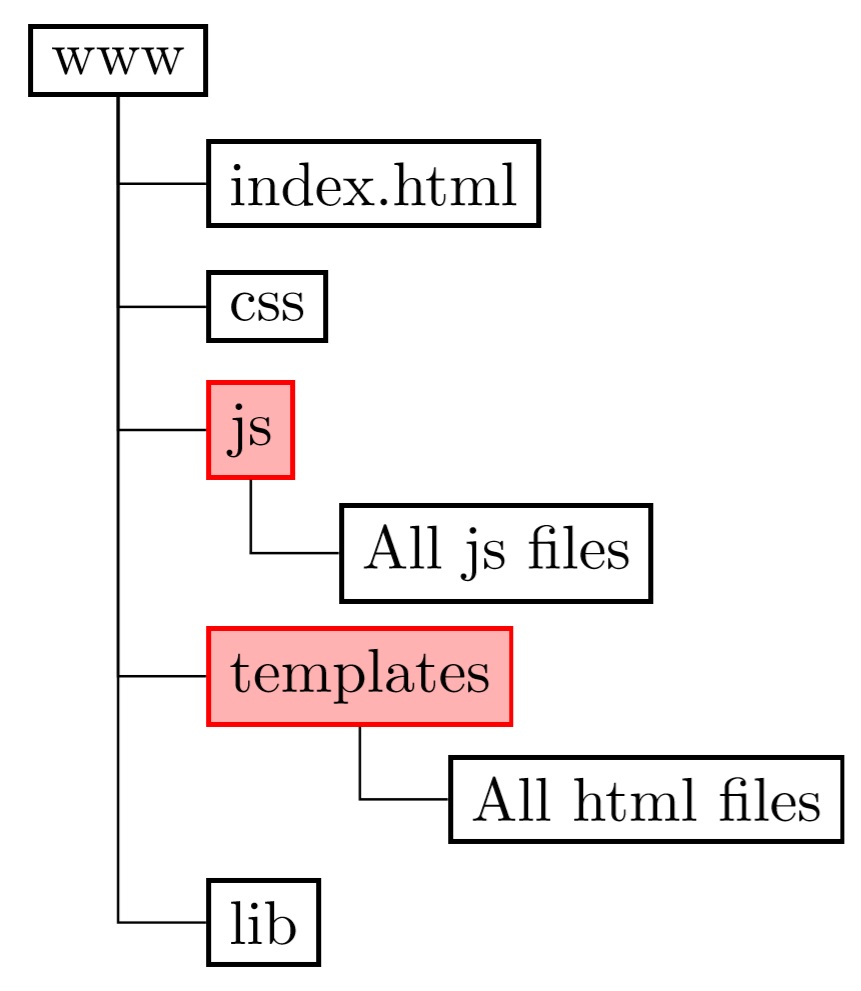
\includegraphics[width=.4\linewidth]{Images/folder_before.jpg}
  \caption{Before}
  \label{fig:before}
\end{subfigure}%
\begin{subfigure}[b]{.5\textwidth}
  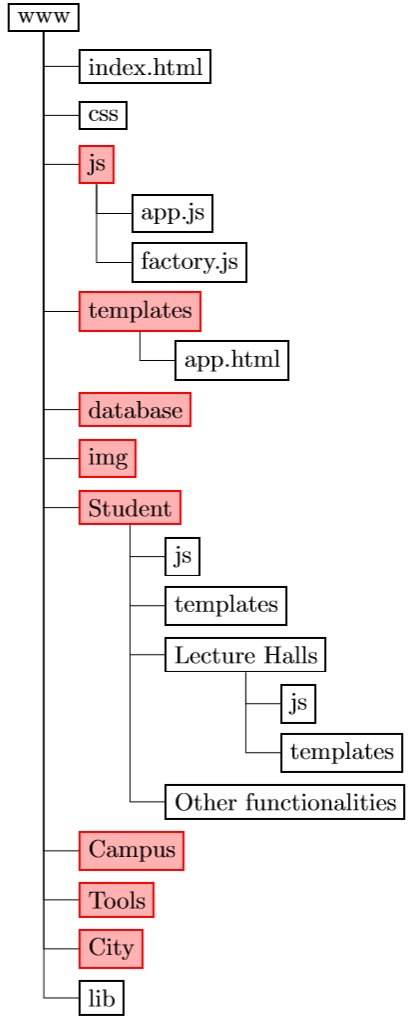
\includegraphics[width=.4\linewidth]{Images/folder_after.jpg}
  \caption{After}
  \label{fig:sub2}
\end{subfigure}
\caption{Folder evolution}
\label{fig:test}
\end{figure}

\subsection{State provider}


\section{Coding standards}

\section{Security}

\section{Information retrieval}
\newpage

\chapter{The application}

In this section we will present the application as we implemented it.

\section{The application UCLCampus}

\subsection{Studies}

\subsection{Campus}

\subsection{City}

\subsection{Tools}

\subsection{Others}


\section{Modularity and how to add a new functionality}


\section{Future functionalities and possible improvements}

\chapter{Analysis}

Here we will reflect about the many choices we made and try to decide wether they were the right ones or not.

\section{Ionic framework}

\section{GitHub}

\section{Project Management}


\chapter{Conclusion} 

\chapter{Bibliography}



\end{document}